\documentclass[final, 24pt]{beamer}

% ====================
% Packages
% ====================

\usepackage[T1]{fontenc}
\usepackage{lmodern}
\usepackage[size=a0,scale=1.2,orientation=portrait]{beamerposter}
\usetheme{gemini}
\usecolortheme{thu}
\usepackage{graphicx}
\usepackage{booktabs}
\usepackage{tikz}
\usepackage{subcaption}
\usepackage{ragged2e}
\usepackage{etoolbox}
\usepackage{microtype}
\usepackage{textcomp}
%\usepackage{mathpazo}
%\usepackage{newpxtext,newpxmath}
\usefonttheme{professionalfonts}
\usefonttheme{serif}
\usepackage{libertine}

% —— 4) 载入与 Libertine 配套的数学字体
\usepackage[libertine]{newtxmath}

% —— 5) 载入 Inconsolata 等宽(tt)字体
\usepackage[scaled=0.85]{inconsolata}
\setmainfont{Libertinus Serif}[Ligatures=TeX,Numbers=OldStyle]
  % “无衬线”也指向 Libertinus Sans,保证一致性
\setsansfont{Libertinus Sans}
  % 等宽字体用 Inconsolata(同样自带)
\setmonofont{Inconsolata}[Scale=0.85]

\AtBeginEnvironment{frame}{\justifying}


\setbeamerfont{caption name}{size=\normalsize}
\setbeamerfont{caption}{size=\normalsize}

% ====================
% Lengths
% ====================

% If you have N columns, choose \sepwidth and \colwidth such that
% (N+1)*\sepwidth + N*\colwidth = \paperwidth
\newlength{\sepwidth}
\newlength{\colwidth}
\setlength{\sepwidth}{0.02\paperwidth}
\setlength{\colwidth}{0.47\paperwidth}

\newcommand{\separatorcolumn}{\begin{column}{\sepwidth}\end{column}}

% ====================
% Title
% ====================

\title{Miresga: Accelerating Layer-7 Load Balancing with Programmable Switches}

\author{Xiaoyi Shi \and Lin He \and Jiasheng Zhou \and Yifan Yang \and Ying Liu }

\institute[shortinst]{ Institue for Network Sciences and Cyberspace, Tsinghua University}

% ====================
% Footer (optional)
% ====================

%\footercontent{
  %\href{https://www.example.com}{https://www.example.com} \hfill
  %ABC Conference 2025, New York --- XYZ-1234 \hfill
  %\href{mailto:alyssa.p.hacker@example.com}{alyssa.p.hacker@example.com}}
% (can be left out to remove footer)

% ====================
% Logo (optional)
% ====================

% use this to include logos on the left and/or right side of the header:
 \logoright{
\includegraphics[height=4cm]{pic/ACM-logo.png}}
 \logoleft{
\includegraphics[height=6cm]{pic/thu-logo.png}}

% ====================
% Body
% ====================

\begin{document}

\begin{frame}[t]
\begin{columns}[t]
\separatorcolumn

\begin{column}{\colwidth}

  \begin{block}{Background \& Motivation}

    Modern online service providers utilize load balancing in cloud data centers to distribute traffic across large server clusters. 
    Typically, these service providers deploy Layer-7 load balancers to correctly distribute traffic to server clusters running different services.

    Figure~\ref{fig:l7lb} shows the architecture of a typical Layer-7 load balancer.
    The load balancer inspects the packet headers and payloads to determine the service type and the corresponding server cluster. Then, it forwards the packets to the selected server cluster.
    \begin{figure}
      \centering
      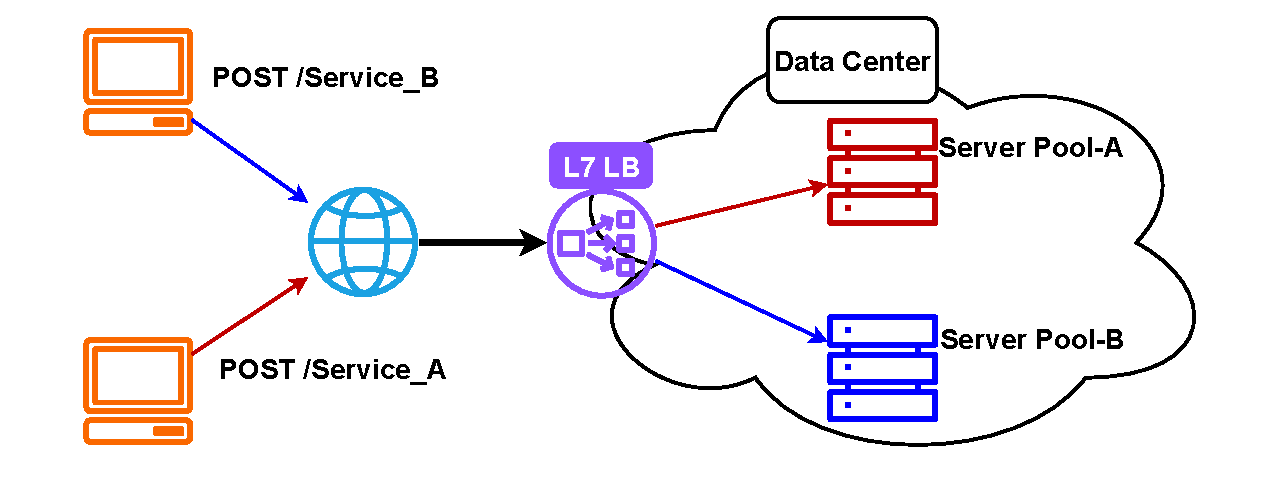
\includegraphics[width=0.9\colwidth]{pic/l7lb.pdf}
      \label{fig:l7lb}
      \caption{The architecture of a typical Layer-7 load balancer.}
    \end{figure}
    However, the increasing demand for high throughput and low latency in cloud data centers has outpaced the capabilities of traditional software Layer-7 load balancers, since the generic CPUs are not optimized for the high-speed packet processing required by Layer-7 load balancing.
    
    The emergence of programmable network hardware, \textit{e.g.}, the programmable switch, has enabled offloading some stateless operations onto the hardware, thereby significantly reducing the load on server CPUs. Programmable switches utilize programmable ASICs to achieve $\sim$Tbps line-rate packet processing, enabling operators to modify packet headers based on customized rules. 
    
    So, our question is that \textcolor{purple}{\fontseries{eb}\selectfont\textbf{can we leverage programmable switches to perform part of the Layer-7 load balancing tasks to replace some server resources?}}

  \end{block}

  \begin{alertblock}{System Overview}

    The core idea of is \textcolor{purple}{\textbf{Hardware-Software Co-design with Proper Layer-7 Load Balancing Partitioning}} to fully leverage the high packet processing speed of programmable switches and the flexible computing capability of CPUs. This co-design is motivated by the strengths and limitations of programmable switches: while they excel in high-speed forwarding, their memory resources and L7 protocol processing capabilities are limited. In contrast, general-purpose servers offer abundant memory resources and strong L7 protocol processing capabilities but lack efficient forwarding performance.
    
    Miresga partitions the Layer-7 load balancing tasks into three sub-tasks and uses three components, the programmable switch, the front-end server, and the back-end agent to handle them:
    \begin{enumerate}
      \justifying
      \item \textcolor{purple}{\textbf{Connection Establishment}}: The programmable switch is responsible for establishing connections and handling SYN packets, while the front-end server is responsible for connection splicing.
      \item \textcolor{purple}{\textbf{Application Protocol Parsing and Decision}}: The front-end server is responsible for parsing the application protocol headers and making routing decisions.
      \item \textcolor{purple}{\textbf{Header Rewriting}}: The programmable switch is responsible for modifying the IP and port, while the back-end agent is responsible for modifying the seq/ack numbers.
    \end{enumerate}

    \begin{figure}
      \centering
      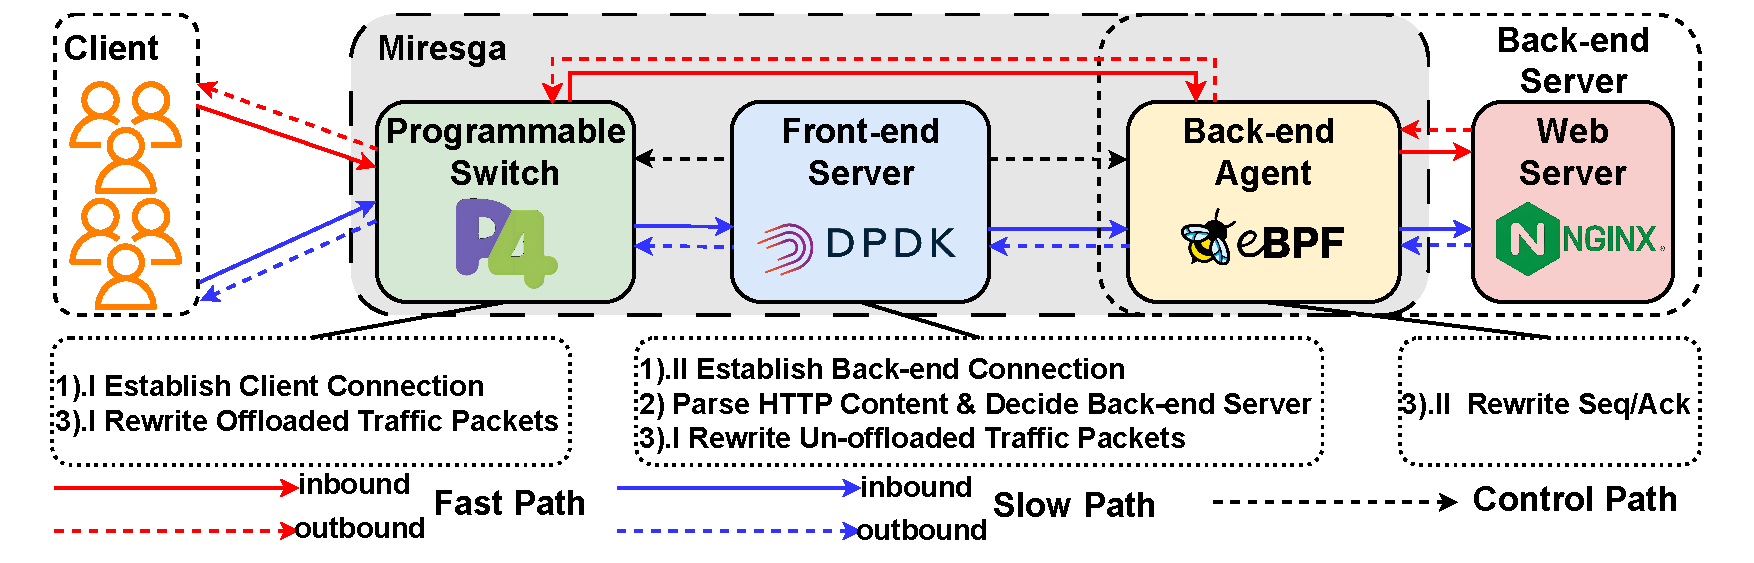
\includegraphics[width=0.9\colwidth]{pic/Miresga_Arch.pdf}
      \label{fig:architecture}
      \caption{The architecture of Miresga}
    \end{figure}

  \end{alertblock}
  \begin{block}{References}

    \nocite{*}
    \footnotesize{\bibliographystyle{plain}\bibliography{poster}}

  \end{block}
  %\begin{minipage}[t]{\paperwidth}
  %    \centering
  %    \begin{figure}
  %        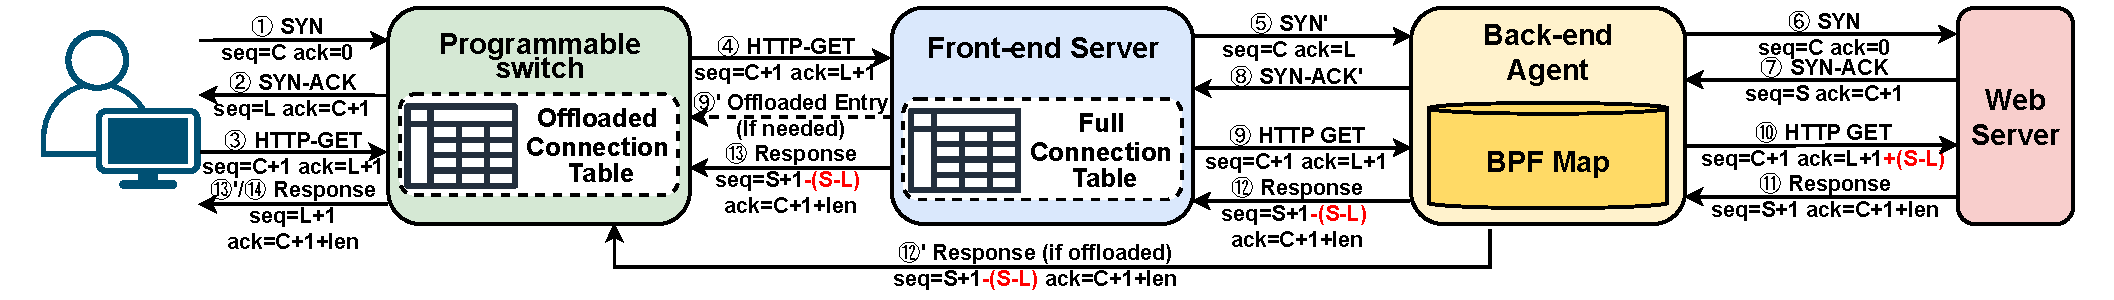
\includegraphics[width=0.9\paperwidth]{pic/Miresga_connection.pdf}
  %    \caption{An Example Workflow of Miresga}
  %    \label{fig:workflow}
  %    \end{figure}
  %\end{minipage}
\end{column}

\separatorcolumn

\begin{column}{\colwidth}

  \begin{alertblock}{Challenges \& Design Details}
  \textcolor{purple}{\textbf{Challenge 1: The finite memory resources inherent in programmable switches limit their ability to accommodate increased traffic volumes.}}

  Firstly, Miresga compresses the stored table entries by merging the two entries corresponding to inbound and outbound traffic, and it employs a single index to obviate the need for storing the complete backend IP and port information. What's more, modifications to the sequence and acknowledgment numbers are delegated to the backend agent that leverages eBPF technology, as this component is not amenable to compression. 

  \textcolor{purple}{\textbf{Challenge 2: The intricate kernel protocol stack contributes to the inefficiency of front-end servers.}}
  
  Miresga employs DPDK technology to bypass the kernel protocol stack and constructs a lightweight protocol stack. Specifically, we consolidate the states of the two connections—between the front-end server and the client, and between the front-end server and the back-end server—into a single flow state. In this design, the front-end server is solely responsible for packet forwarding, while tasks such as retransmission and congestion control are delegated to the client and the back-end servers.

  \begin{figure}
      \centering
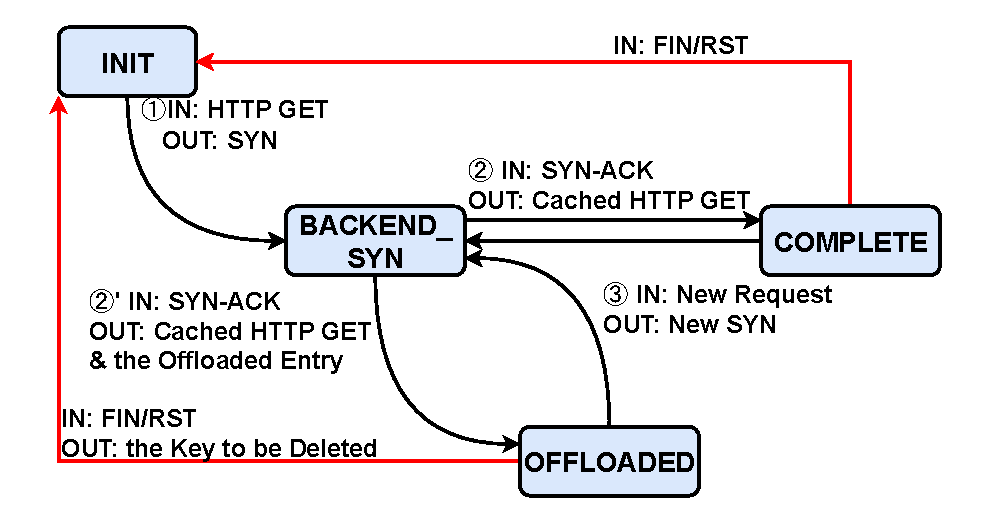
\includegraphics[width=0.8\colwidth]{pic/Miresga_FSM.pdf}
      \caption{The FSM of the lightweight stack.}
      \label{fig:FSM}
  \end{figure}
  
  \textbf{\textcolor{purple}{Challenge 3: State synchronization among the three components introduces additional overhead.}}
  
  In Miresga, two types of states require synchronization: 1) the initial sequence numbers, and 2) the information for splicing connections to the offloaded flows.
  To synchronize the initial sequence number, Miresga fuses the initial sequence numbers into the regular packets to avoid additional delivery. For the latter, Miresga employs an asynchronous synchronization method that does not obstruct traffic flow during the synchronization process. Instead, the front-end server initially handles the traffic, and once synchronization is completed, processing is then transferred to the programmable switch.
  
  
  
  \end{alertblock}

  \begin{block}{Evaluation}
  We primarily evaluated Miresga's end-to-end latency and throughput. The evaluation was conducted across two scenarios: (1) a fixed message size (Figure \ref{fig:fixed_lantency} and Figure \ref{fig:fixed_throughput}), and (2) message sizes generated according to a specific heavy-tailed distribution (Figure \ref{fig:mux_lantency} and Figure \ref{fig:mux_throughput}).
    \begin{figure}
        
        \centering
        \begin{subfigure}[h]{0.48\colwidth}
            \centering
            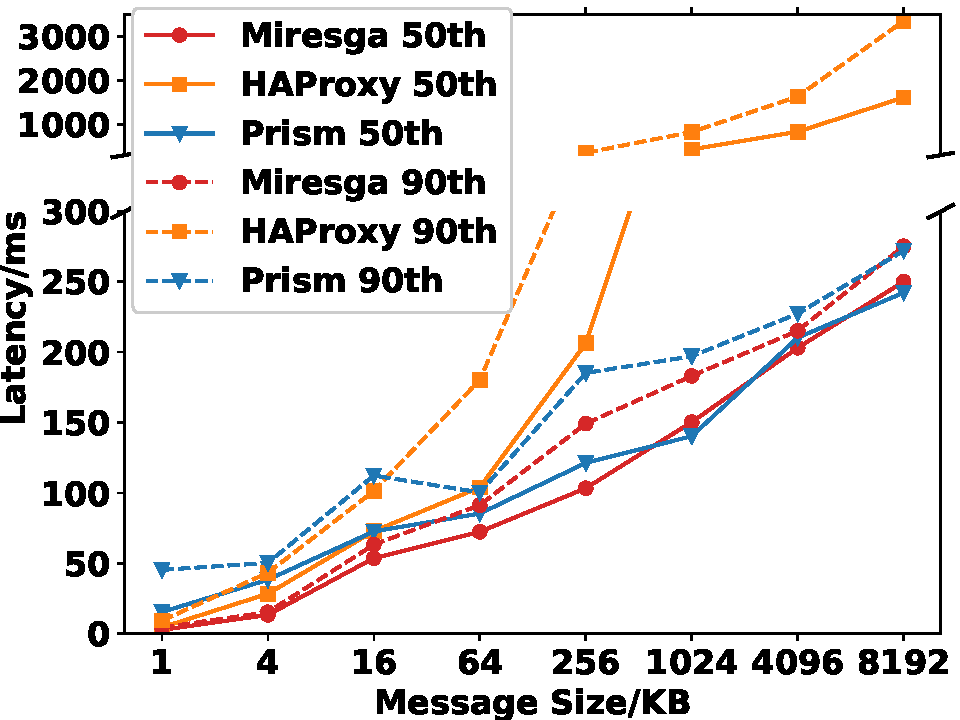
\includegraphics[width=\linewidth]{pic/latency.pdf}
            \caption{Latency with different message sizes}
            \label{fig:fixed_lantency}
        \end{subfigure}
        \begin{subfigure}[h]{0.48\colwidth}
            \centering
            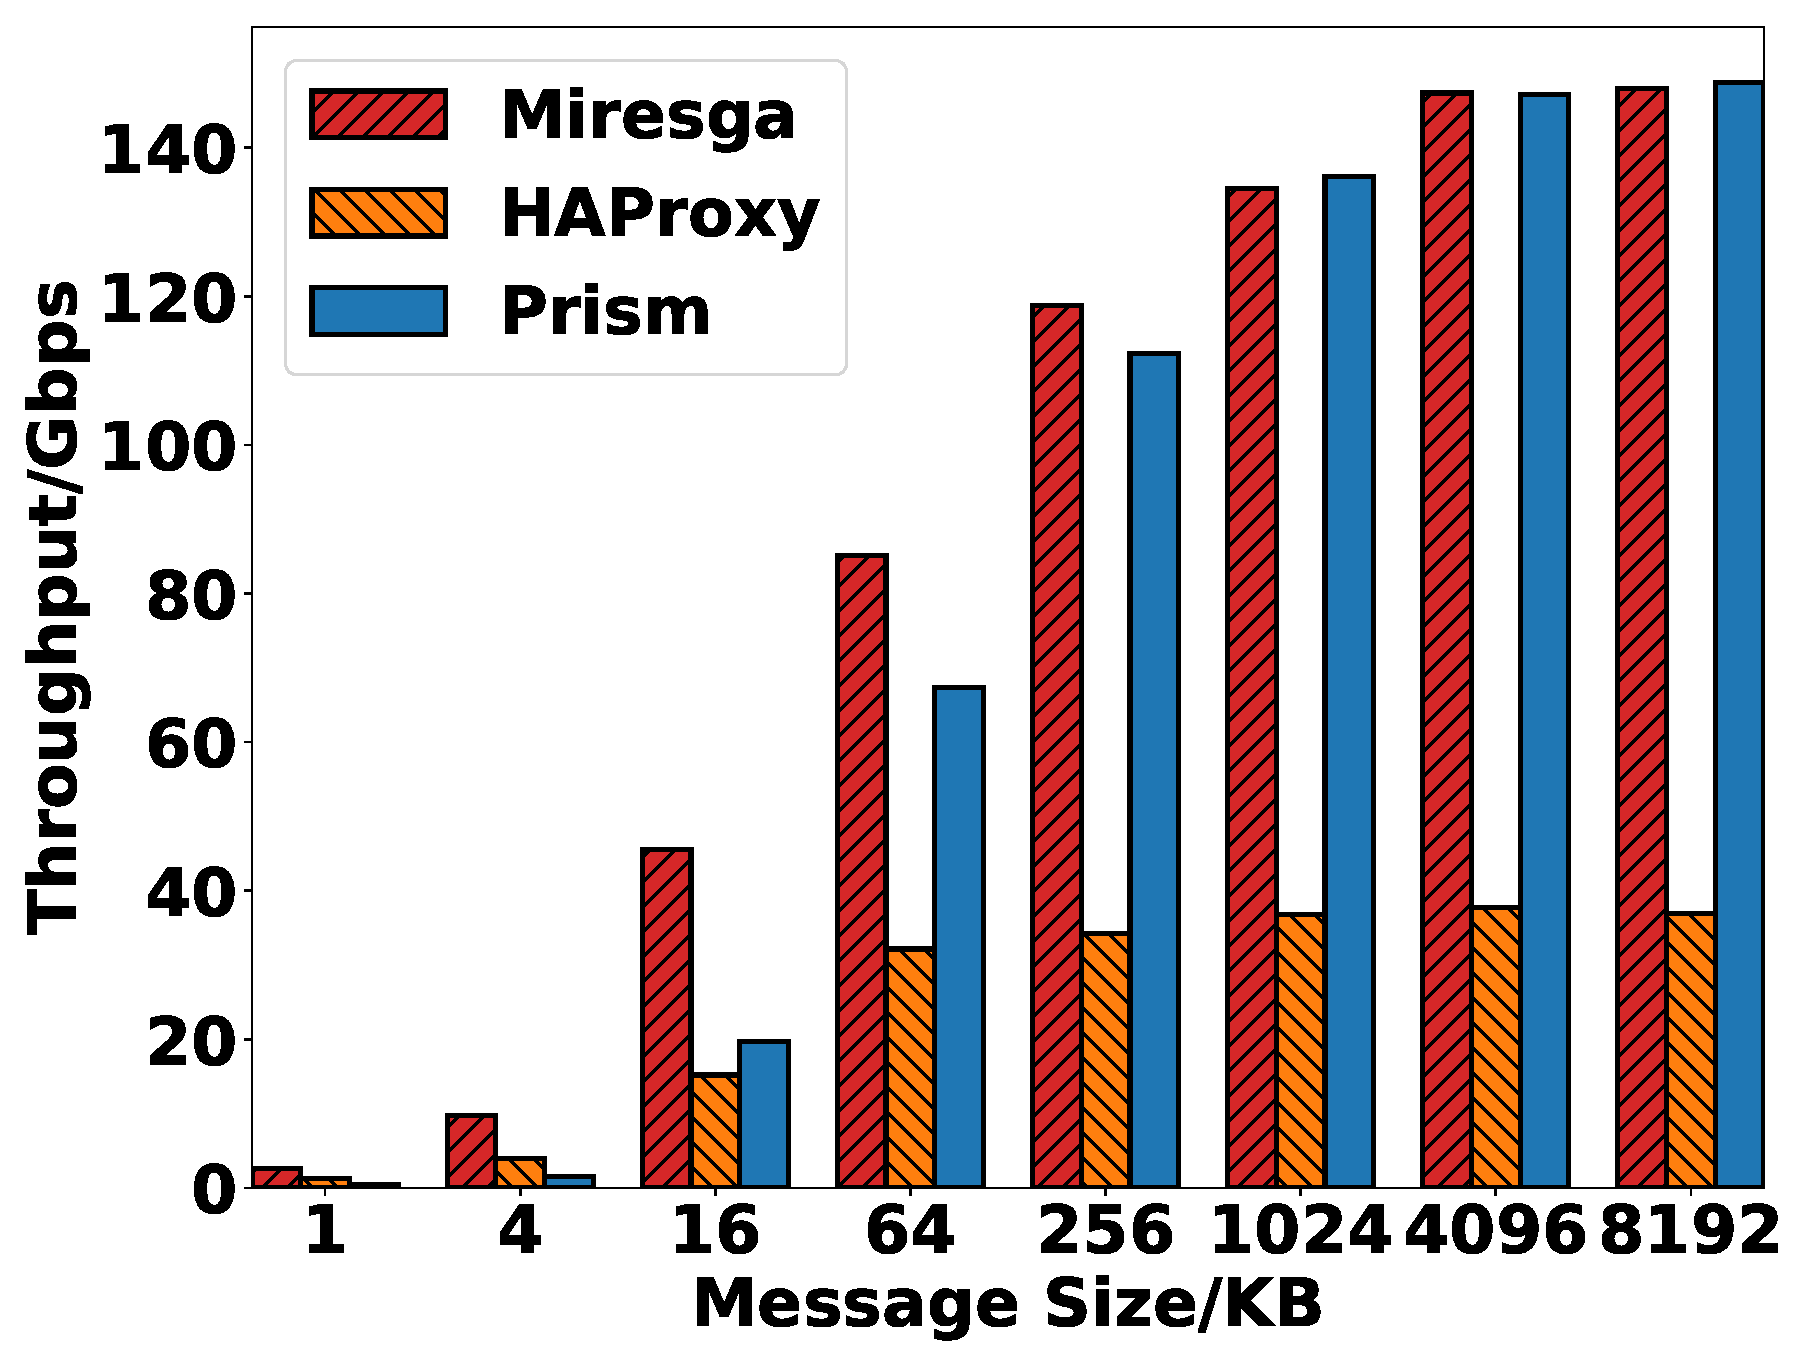
\includegraphics[width=\linewidth]{pic/throughput.pdf}
            \caption{Throughput with different message sizes}
            \label{fig:fixed_throughput}
        \end{subfigure}
        
        \label{fig:fixed}
        \centering
        \begin{subfigure}[h]{0.48\colwidth}
            \centering
            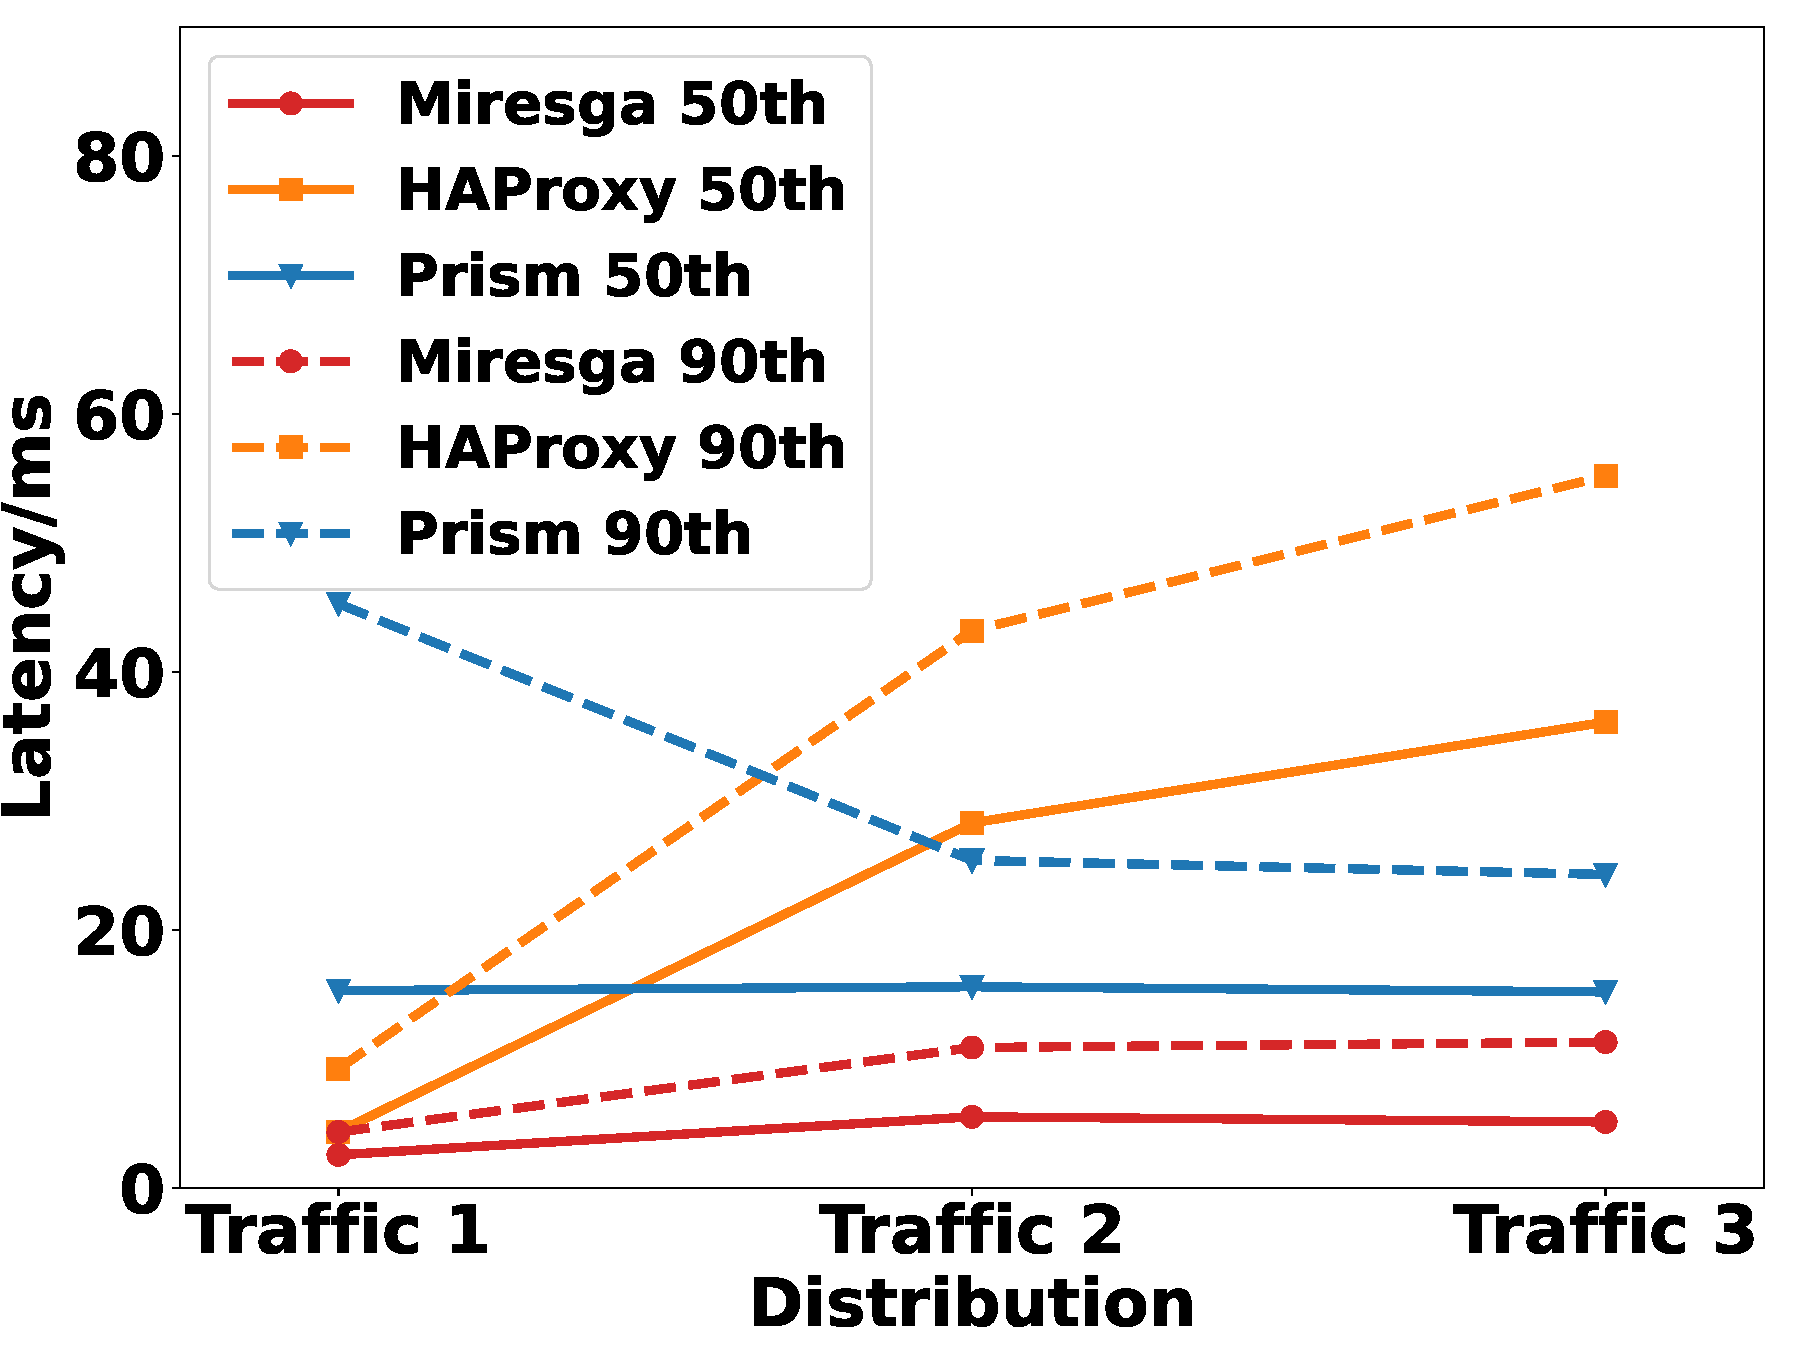
\includegraphics[width=\linewidth]{pic/mux_latency.pdf}
            \caption{\justifying{Latency with heavy-tailed traffic distributions}}
            \label{fig:mux_lantency}
        \end{subfigure}
        \begin{subfigure}[h]{0.48\colwidth}
            \centering
            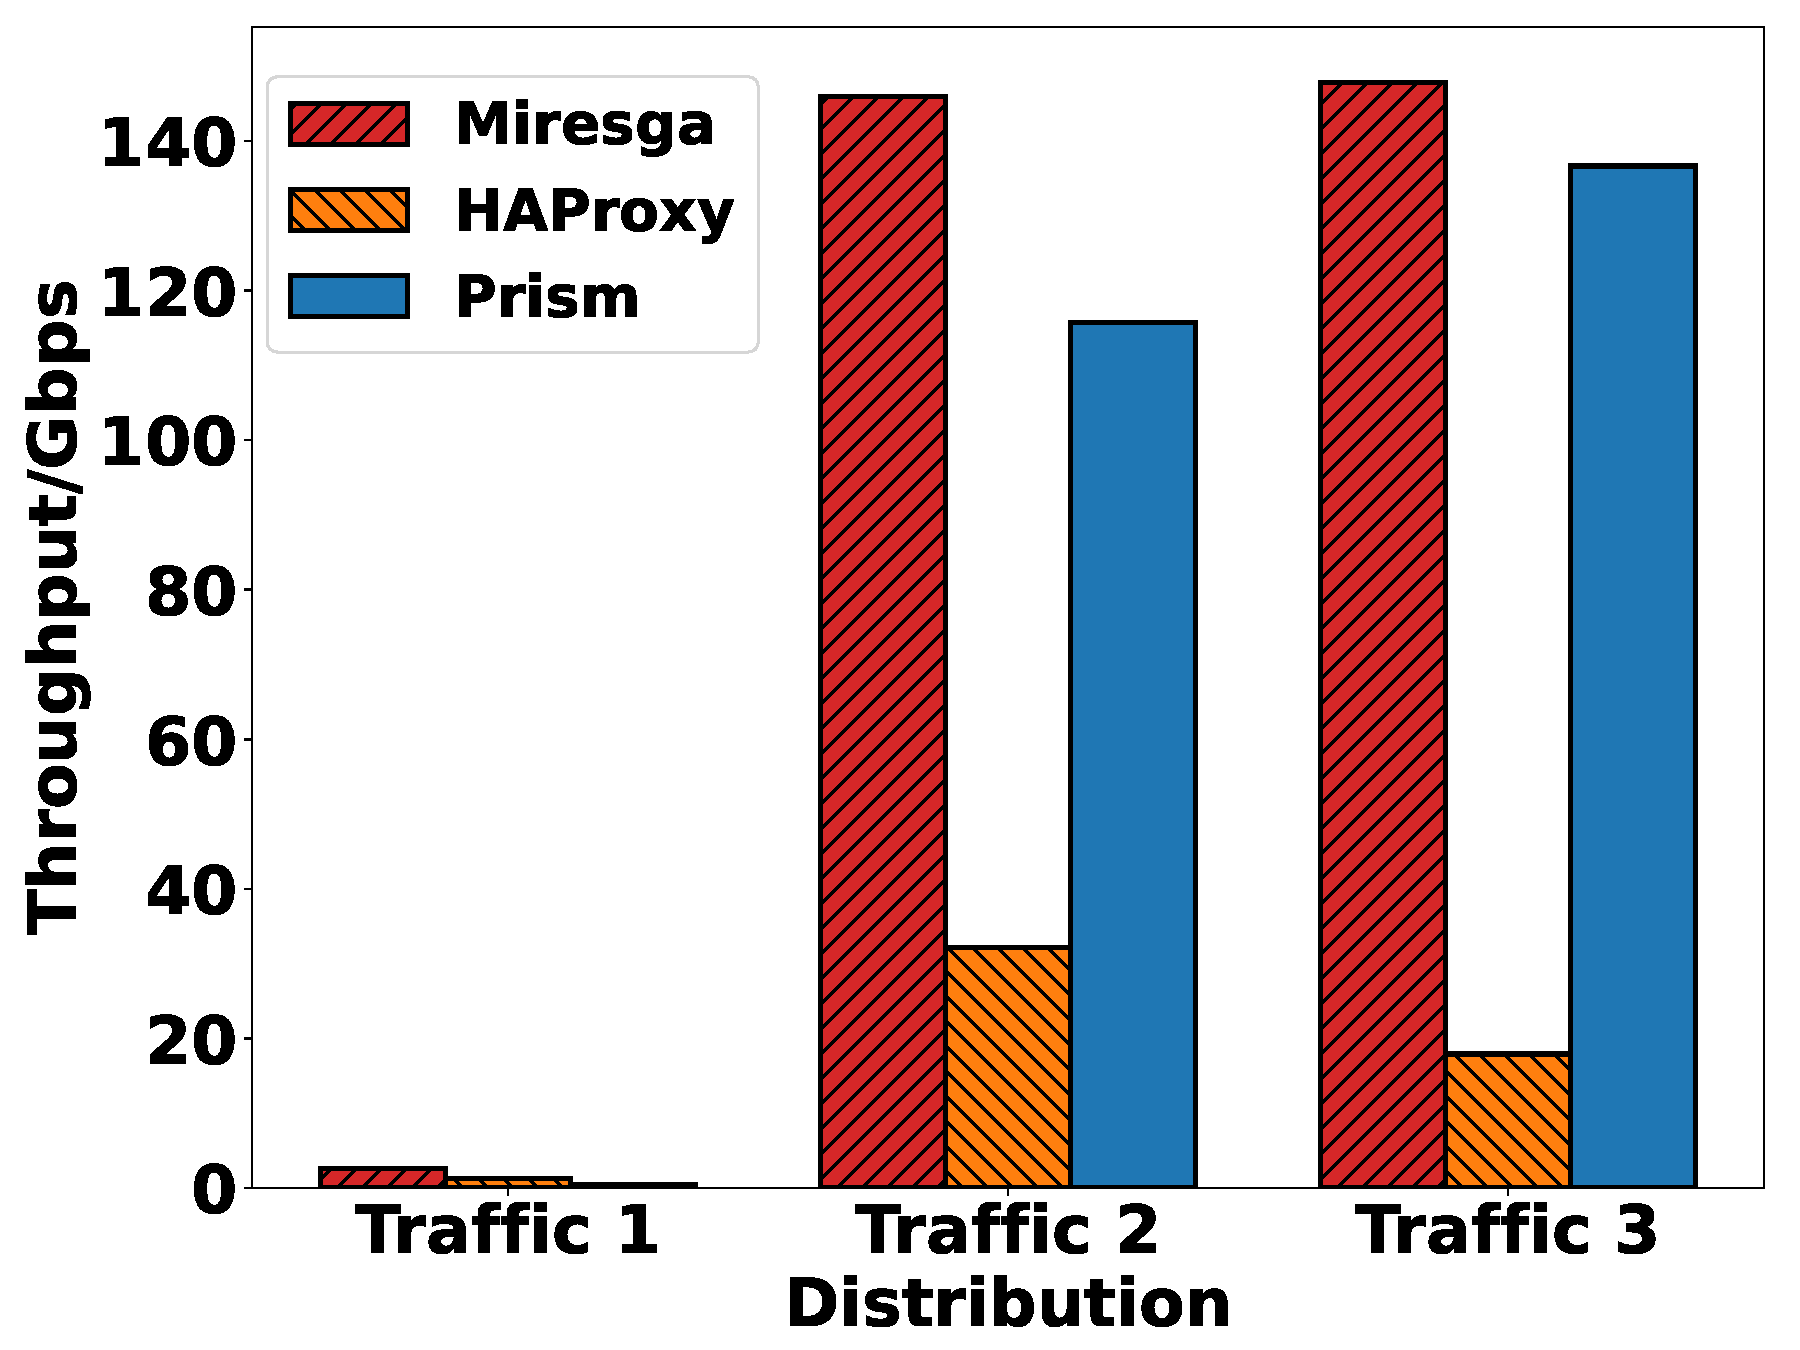
\includegraphics[width=\linewidth]{pic/mux_throughput.pdf}
            \caption{\justifying{Throughput with heavy-tailed traffic distributions}}
            \label{fig:mux_throughput}
        \end{subfigure}
        \caption{\justifying{End-to-end throughput and latency comparison with different message sizes and using heavy-tailed traffic distributions. The distribution of the response size in Traffic 1 is 100\% 1KB; Traffic 2 is 70\% 1KB, 20\% 10KB, 8\% 1MB, and 2\% 10MB. The distribution of the response size in Traffic 2 is 50\% 1KB, 30\% 10KB, 15\% 1MB and 5\% 10MB. We only measure the latency of 1KB message when using heavy-tailed traffic.}}
        \label{fig:e2e}
    \end{figure}
  \end{block}

\end{column}

\separatorcolumn
\end{columns}
\end{frame}

\end{document}
